\documentclass[12pt,a4paper,openany]{article}
\usepackage{lmodern}
\usepackage{xcolor}
\usepackage{xcolor}
\definecolor{vert1}{rgb}{0.0,0.3.9,0.0}
\definecolor{bleu}{rgb}{0,0,0.5}
\definecolor{bleu3}{rgb}{1,0.2,0.2}
\definecolor{grisgris}{gray}{0.4}
\definecolor{rougeUPS}{rgb}{0.6, 0.3, 0.3}

\fboxsep =0pt \parindent =0pt\parskip =12pt



\usepackage[utf8]{inputenc} \usepackage[T1]{fontenc}
\usepackage[francais]{babel}
\usepackage[top=1.7cm, bottom=1.7cm, left=1.7cm, right=1.7cm]{geometry}
\usepackage{verbatim}
\usepackage[urlbordercolor={1 1 1}, linkbordercolor={1 1 1}, linkcolor=vert1, urlcolor=bleu, colorlinks=true]{hyperref}
\usepackage{tikz} %Vectoriel
\usepackage{listings}
\usepackage{fancyhdr}
\usepackage{multido}
\usepackage{float}
\usepackage{amssymb}

\newcommand{\titre}{Dossier de spécifications des besoins logiciels}

\newcommand{\pole}{}
\newcommand{\sigle}{}

\newcommand{\semestre}{4}

\definecolor{gris1}{gray}{0.40}
\definecolor{gris2}{gray}{0.55}
\definecolor{gris3}{gray}{0.65}
\definecolor{gris4}{gray}{0.50}
\definecolor{vert}{rgb}{0,0.4,0}
\definecolor{violet}{rgb}{0.65, 0.2, 0.65}
\definecolor{bleu1}{rgb}{0,0,0.8}
\definecolor{bleu2}{rgb}{0,0.2,0.6}
\definecolor{bleu3}{rgb}{0,0.2,0.2}
\definecolor{rouge}{HTML}{F93928}


\lstdefinelanguage{algo}{%
   morekeywords={%
    %%% couleur 1
		importer, programme, glossaire, fonction, procedure, constante, type, 
	%%% IMPORT & Co.
		si, sinon, alors, fin, tantque, debut, faire, lorsque, fin lorsque, 
		declenche, declencher, enregistrement, tableau, retourne, retourner, =, pour, a,
		/=, <, >, traite,exception, 
	%%% types 
		Entier, Reel, Booleen, Caractere, Réél, Booléen, Caractère,
	%%% types 
		entree, maj, sortie,entrée,
	%%% types 
		et, ou, non,
	},
  sensitive=true,
  morecomment=[l]{--},
  morestring=[b]',
}

\lstset{language=algo,
    %%% BOUCLE, TEST & Co.
      emph={importer, programme, glossaire, fonction, procedure, constante, type},
      emphstyle=\color{bleu2},
    %%% IMPORT & Co.  
	emph={[2]
		si, sinon, alors, fin , tantque, debut, faire, lorsque, fin lorsque, 
		declencher, retourner, et, ou, non,enregistrement, retourner, retourne, 
		tableau, /=, <, =, >, traite,exception, pour, a
	},
      emphstyle=[2]\color{bleu1},
    %%% FONCTIONS NUMERIQUES
      emph={[3]Entier, Reel, Booleen, Caractere, Booléen, Réél, Caractère},
      emphstyle=[3]\color{gris1},
    %%% FONCTIONS NUMERIQUES
      emph={[4]entree, maj, sortie, entrée},	
      emphstyle=[4]\color{gris1},
}
\lstdefinelanguage{wl}{%
   morekeywords={%
    %%% couleur 1
		importer, programme, glossaire, fonction, procedure, constante, type, 
	%%% IMPORT & Co.
		si, sinon, alors, fin, TANTQUE, tantque, FIN, PROCEDURE, debut, faire, lorsque, 
		fin lorsque, declenche, declencher, enregistrement, tableau, retourne, retourner, =, 
		/=, <, >, traite,exception, 
	%%% types 
		Entier, Reel, Booleen, Caractere, Réél, Booléen, Caractère,
	%%% types 
		entree, maj, sortie,entrée,
	%%% types 
		et, ou, non,
	},
  sensitive=true,
  morecomment=[l]{//},
  morestring=[b]',
}

\lstset{language=wl,
    %%% BOUCLE, TEST & Co.
      emph={importer, programme, glossaire, fonction, procedure, constante, type},
      emphstyle=\color{bleu2},
    %%% IMPORT & Co.  
	emph={[2]
		si, sinon, alors, fin , tantque, debut, faire, lorsque, fin lorsque, 
		declencher, retourner, et, ou, non,enregistrement, retourner, retourne, 
		tableau, /=, <, =, >, traite,exception
	},
      emphstyle=[2]\color{bleu1},
    %%% FONCTIONS NUMERIQUES
      emph={[3]Entier, Reel, Booleen, Caractere, Booléen, Réél, Caractère},
      emphstyle=[3]\color{gris1},
    %%% FONCTIONS NUMERIQUES
      emph={[4]entree, maj, sortie, entrée},	
      emphstyle=[4]\color{gris1},
}
\lstdefinelanguage{css}{%
   morekeywords={%
    %%% couleur 1
		background, image, repeat, position, index, color, border, font, 
		size, url, family, style, variant, weight, letter, spacing, line, 
		height, text, decoration, align, indent, transform, shadow, 
		background, image, repeat, position, index, color, border, font, 
		size, url, family, style, variant, weight, letter, spacing, line, 
		height, text, decoration, align, indent, transform, shadow, 
		vertical, align, white, space, word, spacing,attachment, width, 
		max, min, margin, padding, clip, direction, display, overflow,
		visibility, clear, float, top, right, bottom, left, list, type, 
		collapse, side, empty, cells, table, layout, cursor, marks, page, break,
		before, after, inside, orphans, windows, azimuth, after, before, cue, 
		elevation, pause, play, during, pitch, range, richness, spek, header, 
		numeral, punctuation, rate, stress, voice, volume,
	%%% types 
		left, right, bottom, top, none, center, solid, black, blue, red, green,
	},
  sensitive=true,
  sensitive=true,
  morecomment=[s]{/*}{*/},
  morestring=[b]',
}
\lstset{language=css,
    %%% BOUCLE, TEST & Co.
      emph={
		background, image, repeat, position, index, color, border, font, 
		size, url, family, style, variant, weight, letter, spacing, line, 
		height, text, decoration, align, indent, transform, shadow, 
		background, image, repeat, position, index, color, border, font, 
		size, url, family, style, variant, weight, letter, spacing, line, 
		height, text, decoration, align, indent, transform, shadow, 
		vertical, align, white, space, word, spacing,attachment, width, 
		max, min, margin, padding, clip, direction, display, overflow,
		visibility, clear, float, top, right, bottom, left, list, type, 
		collapse, side, empty, cells, table, layout, cursor, marks, page, break,
		before, after, inside, orphans, windows, azimuth, after, before, cue, 
		elevation, pause, play, during, pitch, range, richness, spek, header, 
		numeral, punctuation, rate, stress, voice, volume,
	  },
      emphstyle=\color{bleu2},
    %%% FONCTIONS NUMERIQUES
      emph={[3]
		left, right, bottom, top,none, solid, black, blue, green,
		  },
      emphstyle=[3]\color{bleu3},
    %%% FONCTIONS NUMERIQUES
}

\lstset{language=SQL,
    %%% BOUCLE, TEST & Co.
      emph={INSERT, UPDATE, DELETE, WHERE, SET, GROUP, BY, ORDER},
      emphstyle=\color{bleu2},
    %%% IMPORT & Co.  
	emph={[2]
		if, end, begin, then, for, each, else, after, of, on, to
	},
      emphstyle=[2]\color{bleu1},
    %%% FONCTIONS NUMERIQUES
      emph={[3]Entier, Reel, Booleen, Caractere, Booléen, Réél, Caractère},
      emphstyle=[3]\color{gris1},
    %%% FONCTIONS NUMERIQUES
      emph={[4]entree, maj, sortie, entrée},	
      emphstyle=[4]\color{gris1},
}
\lstdefinelanguage{ARM}{%
   morekeywords={%
   ADD, SUB, MOV, MUL, RSB,CMP, BLS, BLE, B,BHI,
   BGE, RSBLT, BGT, BEQ, BNE,BLT
	},
  sensitive=true,
  morecomment=[l]{@},
  morestring=[b]',
}

\lstset{ % general style for listings 
   numbers=left 
   , literate={é}{{\'e}}1 {è}{{\`e}}1 {à}{{\`a}}1 {ê}{{\^e}}1 {É}{{\'E}}1 {ô}{{\^o}}1 {€}{{\euro}}1{°}{{$^{\circ}$}}1 {ç}{ {c}}1
	, extendedchars=\true
   , tabsize=2 
   , frame=l
   , framerule=1.1pt
   , linewidth=520px
   , breaklines=true 
   , basicstyle=\footnotesize\ttfamily 
   , numberstyle=\tiny\ttfamily 
   , framexleftmargin=0mm 
   , xleftmargin=0mm 
   , captionpos=b 
	, keywordstyle=\color{bleu2}
	, commentstyle=\color{vert}
	, stringstyle=\color{rouge}
	, showstringspaces=false
	, extendedchars=true
	, mathescape=true
} 
%	\lstlistoflistings
%	\addcontentsline{toc}{part}{List of code examples}

\date{\today}

\makeindex
\lfoot{Université Toulouse III -- Paul Sabatier}
\rfoot{}
%\rfoot{}
\cfoot{}
\makeglossary
\makeatletter
\def\clap#1{\hbox to 0pt{\hss #1\hss}}%
\def\ligne#1{%
\hbox to \hsize{%
\vbox{\centering #1}}}%
\def\haut#1#2#3{%
\hbox to \hsize{%
\rlap{\vtop{\raggedright #1}}%
\hss
\clap{\vtop{\centering #2}}%
\hss
\llap{\vtop{\raggedleft #3}}}}%
\def\bas#1#2#3{%
\hbox to \hsize{%
\rlap{\vbox{\raggedright #1}}%
\hss \clap{\vbox{\centering #2}}%
\hss
\llap{\vbox{\raggedleft #3}}}}%
\def\maketitle{%
\thispagestyle{empty}\vbox to \vsize{%
\haut{}{\@blurb}{}

\vfill
\vspace{1cm}
\begin{flushleft}
\usefont{OT1}{ptm}{m}{n}
\huge \@title
\end{flushleft}
\par
\hrule height 4pt
\par
\begin{flushright}
\usefont{OT1}{phv}{m}{n}
\Large \@author
\par
\end{flushright}
\vspace{1cm}
\vfill
\vfill
\bas{}{\@location, le \@date}{}
}%
\cleardoublepage
}
\def\date#1{\def\@date{#1}}
\def\author#1{\def\@author{#1}}
\def\title#1{\def\@title{#1}}
\def\location#1{\def\@location{#1}}
\def\blurb#1{\def\@blurb{#1}}
\date{\today}
\author{}
\title{}
\location{Amiens}\blurb{}
\makeatother
\title{\titre}
\author{Projet de Boggle}

\location{Toulouse}
\blurb{%
Université Toulouse III -- Paul sabatier\\
L2 Informatique\\
Projet tuteuré\\
\vspace{30px}
\begin{flushleft}Antoine de \bsc{Roquemaurel}\\ Fabrice
	\bsc{Valleix}\\ Groupe 2.2\end{flushleft}
}%



%\title{Cours \\ \titre}
%\date{\today\\ Semestre \semestre}

%\lhead{Cours: \titre}
%\chead{}
%\rhead{\thepage}

%\lfoot{Université Paul Sabatier Toulouse III}
%\cfoot{\thepage}
%\rfoot{\sigle\semestre}

\pagestyle{fancy}
%\renewcommand{\chaptermark}[1]{\markboth{\bsc{\chaptername~\thechapter{} :} #1}{}}
\renewcommand{\sectionmark}[1]{\markright{\thesection{ #1}}}
\renewcommand{\headrulewidth}{0.3pt}
\renewcommand{\footrulewidth}{0.3pt}

\fancyhf{}
\fancyhead[LO]{Antoine de \bsc{Roquemaurel} -- Fabrice \bsc{Valleix}}
\fancyhead[RO]{\rightmark}
\fancyfoot[CO]{--~\thepage~--}
\fancyfoot[LO]{Dossier de spécifications}
\fancyfoot[RO]{Projet de Boggle}
\fancyfoot[RE]{Antoine de \bsc{Roquemaurel} -- Fabrice \bsc{Valleix}}

%% Cas des premières pages de chapitre
\fancypagestyle{plain}{%
	\fancyhf{}%
	\fancyfoot[L]{\titre{}}
	\fancyfoot[R]{--~\thepage~--}
	\renewcommand{\headrulewidth}{0pt}
	\renewcommand{\footrulewidth}{0.3pt}
}
\makeatletter
\renewcommand*{\lstlistlistingname}{Liste des codes sources}
\renewcommand{\listfigurename}{Liste des figures}
\renewcommand\listoffigures{%
    \subsection{\listfigurename}%
      \@mkboth{\MakeUppercase\listfigurename}%
              {\MakeUppercase\listfigurename}%
       \@starttoc{lof}%
    }
    \renewcommand\listoftables{%
    \subsection{\listtablename}%
    \@mkboth{\MakeUppercase{\listtablename}}%
            {\MakeUppercase{\listtablename}}%
    \@starttoc{lot}
    }

    \renewcommand\lstlistoflistings{%
    \begingroup
    \subsection{\lstlistlistingname}%
    \parskip\z@\parindent\z@\parfillskip \z@ \@plus 1fil%
    \@starttoc{lol}%
    \endgroup
    }
	\makeatother

\definecolor{exemple}{HTML}{dde5ed}
\definecolor{remarque}{HTML}{dde5ed}
\newcommand{\exemple}[1]{
	\begin{center}
	\medskip
	\colorbox{exemple}{
	\begin{minipage}{0.8\textwidth}\vspace{10px}\textbf{Ex }\medskip#1 \medskip\end{minipage}
	}
	\medskip
	\end{center}
}
\newcommand{\remarque}[1]{
	\begin{center}
	\medskip
	\colorbox{remarque}{
		\begin{minipage}{0.8\textwidth}\medskip\includegraphics[height=10px]{/home/aroquemaurel/cours/includesLaTeX/images/remarque.png} #1 \medskip\end{minipage}
	}
	\medskip
	\end{center}
}

\newcommand{\attention}[1]{
	\begin{center}
	\medskip
	\colorbox{remarque}{
		\begin{minipage}{0.8\textwidth}\medskip\includegraphics[height=10px]{/home/aroquemaurel/cours/includesLaTeX/images/attention.png} #1 \medskip\end{minipage}
	}
	\medskip
	\end{center}
}

\DeclareTextFontCommand{\policeGlossaire}{\fontfamily{lmss}\selectfont}
\DeclareTextFontCommand{\policePackage}{\fontfamily{phv}\selectfont}
\DeclareTextFontCommand{\policeTitre}{\fontfamily{ptm}\selectfont}
\newcommand{\policeCode}[1]{\texttt{#1}}

\newcommand{\sectionfont}{%
	\fontencoding{\encodingdefault}%
	\fontfamily{pag}%
	\fontseries{bc}%
	\fontshape{n}%
	\selectfont
}

% numéro du chapitre
\DeclareFixedFont{\chapnumfont}{T1}{phv}{b}{n}{80pt}
% pour le mot « Chapitre »
\DeclareFixedFont{\chapchapfont}{T1}{phv}{b}{n}{16pt}
% pour le titre
\DeclareFixedFont{\chaptitfont}{T1}{phv}{b}{n}{24.88pt}


\makeatletter
\def\thickhrulefill{\leavevmode \leaders \hrule height 1ex \hfill \kern \z@}

\newlength{\sectiontitleindent}
\newlength{\subsectiontitleindent}
\newlength{\subsubsectiontitleindent}
\setlength{\sectiontitleindent}{-1cm}
\setlength{\subsectiontitleindent}{-.5cm}
\setlength{\subsubsectiontitleindent}{-.25cm}

\renewcommand{\section}{%
	\@startsection%
	{section}%
	{1}%
	{\sectiontitleindent}%
	{-3.5ex plus -1ex minus -.2ex}%
	{2.3ex plus.2ex}%
	{\sectionfont\Large}
}
\renewcommand{\subsection}{%
	\@startsection%
	{subsection}%
	{2}%
	{\subsectiontitleindent}%
	{-3.5ex plus -1ex minus -.2ex}%
	{2.3ex plus.2ex}%
	{\sectionfont\large}
}

\renewcommand{\subsubsection}{%
	\@startsection%
	{subsubsection}%
	{3}%
	{\subsubsectiontitleindent}%
	{-3.5ex plus -1ex minus -.2ex}%
	{2.3ex plus.2ex}%
	{\sectionfont\normalsize}
}

\makeatother

\newcommand{\lien}[1]{
 $\vartriangleright$ \url{#1}
 }

\newcommand{\pfp}{\texttt{pfp}}

\newcommand{\ifp}{\texttt{if}}
\newcommand{\elsep}{\texttt{else}}

\makeatother
\includeonly {
}
\begin{document}
	\setcounter{tocdepth}{2}
	\setcounter{secnumdepth}{3}
	\maketitle
	\tableofcontents
	\newpage
	\section{Avant-propos}
		\subsection{But du document}
	Le but de ce document est de lister toutes les fonctionnalités du futur logiciel et de son contexte d’utilisation (utilisateurs, autres composantes,
	matériel,  etc.).
		\subsection{Contexte de l'application}
		Cette application sera développé par Antoine de \bsc{Roquemaurel} et Fabrice \bsc{Valleix} dans le cadre du projet logiciel du 
		semestre 4 de la L2 Informatique de l'université Toulouse III -- Paul Sabatier.
	
	\section{Description globale} 
	Le logiciel sera un jeu de Boggle$^{\tiny\textregistered}$.

	Le jeu prend la forme d'une grille carrée, la taille étant donné par l'utilisateur. Dans chaque case de la grille est présente une lettre, au
	commencement du jeu, un compte à rebours de trois minutes est lancé, durant ces trois minutes le joueur doit chercher le plus de mots pouvant être
	formés à partir de lettre adjacentes du plateau, les mots peuvent doivent être de plus de 3 lettres et être présent dans le dictionnaire afin d'être
	acceptés.
	\subsection{Environnement}
		Le logiciel pourra être utilisé sur un ordinateur classique, sous GNU/Linux, aucun matériel externe ne sera nécessaire au bon fonctionnement du
		programme, de même le serveur d'interface graphique \texttt{X} ne sera pas utile, en effet le programme fonctionnera en mode texte ou semi graphique.
	\subsection{Profil des utilisateurs}
		Le logiciel possédera un unique profil d'utilisateur.
		\begin{description}
			\item[Le joueur] Il veut faire une partie de Boggle pour s'amuser ou passer le temps. L'ordinateur génère une grille de Boggle puis le
				joueur cherche des mots pendant 3 minutes en essayant de faire le plus de points possible. Il peut éventuellement défier un ami afin de
				savoir lequel des deux obtiendra le plus de points.
		\end{description}

	\section{Spécifications générales}
	\subsection{Description des services attendus}
	Les servies attendus de l'application sont au nombres de deux.
		\begin{description}
			\item[Résoudre une grille par l'ordinateur] L'application doit être capable de résoudre une grille de Boggle, ceci peut importe la taille de
				la grille.
			\item[Effectuer une partie]  Et enfin, l'utilisateur devra pouvoir effectuer une partie de Boggle.
		\end{description}
	\subsection{Description générale des fonctions}
	Les fonctions sont réparties en deux catégories: celle qui seront utilisés pour la résolution d'une grille et celle indispensable pour effectuer
	une partie de Boggle.
	\subsubsection{Effectuer une partie de Boggle}
		\begin{description}
				\item[Génération d'une grille] L'application doit pouvoir générer une grille de Boggle, celle-ci devra être adapté à la langue Française, en
				effet les lettres auront des probabilités d'apparaître en fonction de leur utilisation en Français, ceci afin d'éviter les grilles où
				l'utilisateur ne peut rien faire.
				\item[Lancer le compte à rebours] Au départ de la partie, un compte à rebours de trois minutes doit être lancé, à la fin des trois
					minutes, l'utilisateur ne peut plus proposer de nouveau mot.
				\item[Proposition d'un mot] L'utilisateur peut proposer un mot, l'ordinateur l'accepte ou le refuse en fonction des critères suivants:
					\begin{itemize}
						\item Présent dans la langue Française
						\item Longueur du mot supérieur ou égal à 3
						\item Suite de lettre dans la grille
						\item Mot non déjà utilisé
					\end{itemize}
				\item[Calcul du nombre de points obtenus] À la fin d'une partie, l'application doit afficher le nombre de points du joueur, et le
					nombre de points qu'il aurait pus faire s'il avait découvert l'intégralité des mots présents dans la grille, plus un mot est long
					plus il rapporte de points. Les points sont calculés ainsi:
					\begin{itemize}
						\item 3 et 4 lettres : 1 point
						\item 5 lettres : 2 points
						\item 6 lettres : 3 points
						\item 7 lettres : 5 points
						\item 8 lettres et plus : 11 points
					\end{itemize}
		\end{description}
	\subsubsection{Résoudre une grille de Boggle}
		\begin{description}
			\item[Résoudre une grille par l'ordinateur] 
				L'application doit être capable de résoudre une grille de Boggle afin de pouvoir afficher la solution à l'utilisateur une foi qu'il a
				finis une partie. Pour cela il doit afficher tous les mots qui aurait pus être trouvés.
			\item[Demande d'aide pour une lettre donnée] Pour une lettre donné, l'application doit afficher la longueur du mot le plus long qui
				commence par les lettres sélectionnés.
			\item[Affichage de la solution] 
				Afin d'afficher la solution l'application utilisera son résolveur. Il résout la grille et afficher ensuite tous les mots qui sont
				présent dans la grille avec les point correspondants.
		\end{description}
		\begin{figure}[H]
			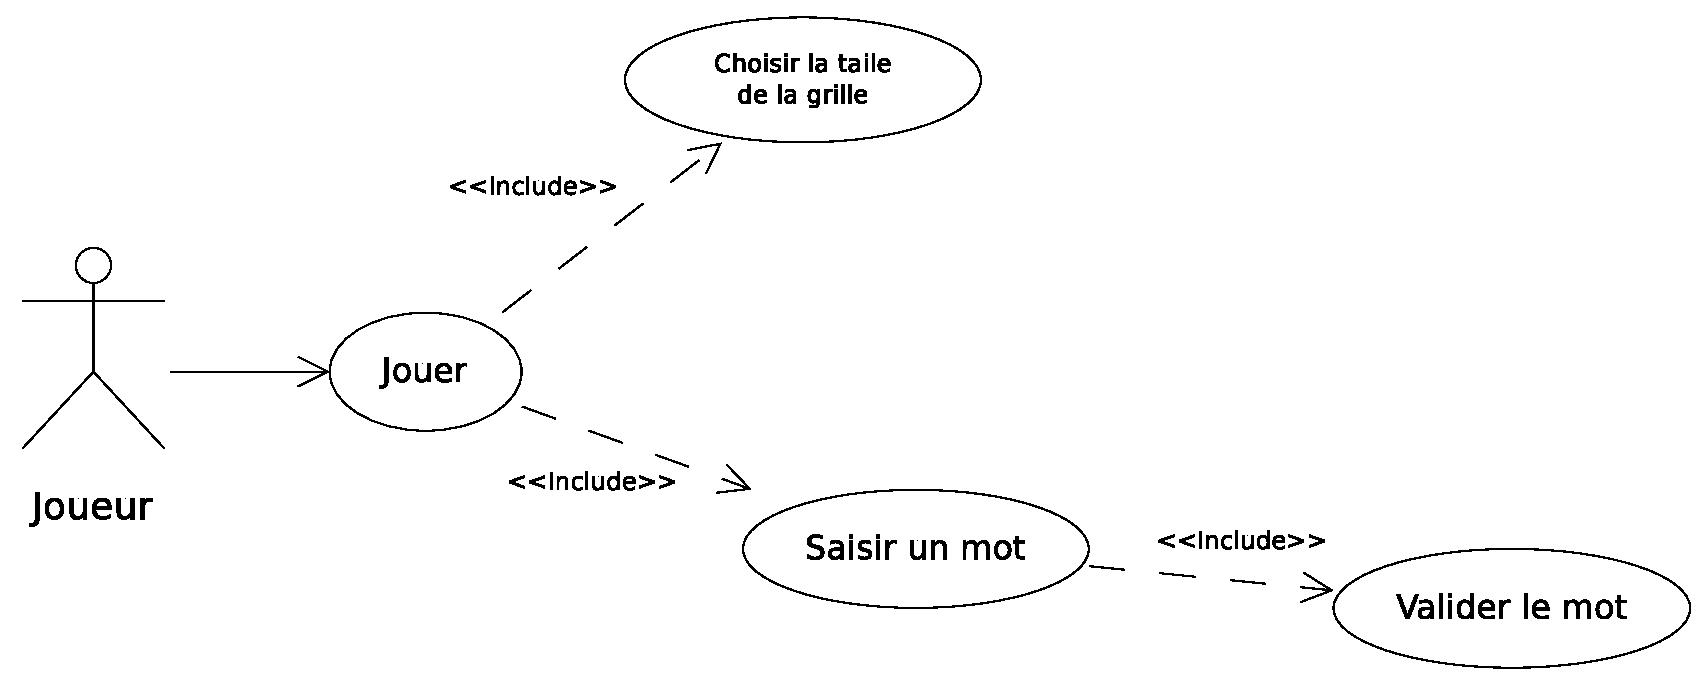
\includegraphics[width=15cm]{usecase.eps}
			\caption{Diagramme de cas d'utilisations}
		\end{figure}

	\section{Exigences opérationnelles} % TODO
	\subsection{Contrainte d'exploitation}
	\subsection{Modes de fonctionnement}
	Le logiciel disposera de deux modes de fonctionnement différents :
	\begin{itemize}
		\item Le mode texte
		\item Le mode pseudo graphique
	\end{itemize}
	Ces deux modes seront choisis en fonction des arguments du programme, par défaut l'application sera lancée avec le mode pseudo graphique.
	\subsection{Capacités}
		% 
	\subsection{Performances}
		% 

	\section{Scénarii d'utilisations}
		% Faire une partie (3 minutes)
			% Demander la taille de la grille
				% Taille n'est pas bonne
					% out
			% Générer grille
			% lancer timer
			% Proposer mots
				% si mot correct
					% calculer point
				% sinon, rejeter le mot et afficher message
			% timer claque
				% Calculer nombre de point total
				% Afficher mots manquants
\end{document}

